\documentclass[12pt]{article}

% Packages
\usepackage[utf8]{inputenc} % allow utf-8 input
\usepackage[T1]{fontenc}    % use 8-bit T1 fonts
\usepackage{geometry}       % to change the page dimensions
\usepackage{graphicx}       % support the \includegraphics command and options
\usepackage{amsmath}        % for better mathematical formulas
\usepackage{amsfonts}       % for mathematical fonts
\usepackage{amssymb}        % for mathematical symbols
\usepackage{hyperref}       % for hyperlinks
\usepackage{lipsum}         % for generating filler text
\usepackage{float}          % for better figure placement
\usepackage{natbib}         % for better citations
\usepackage{pdfpages}       % for including pdfs
\bibliographystyle{unsrtnat}

% Page geometry
\geometry{a4paper, margin=1in}

\begin{document}

%Title Page
\begin{titlepage}
    \centering
    \vspace*{5cm}

    \Large
    \textbf{Multi-Agent SLAM: Exploration and Mapping in Simulated testing Environments}

    \vspace{1cm}

    Charlie Anthony [CandNo: 246537]\\
    Supervisor: Dr Chris Johnson



    \vfill

    \vspace{1cm}

    \small
    Dissertation\\
    Computer Science and Artificial Intelligence BSc

    
\includegraphics[width=0.3\linewidth]{sussex_logo.jpg}


    \small
    Department of Informatics and Engineering\\
    University of Sussex\\
    May 2024
\end{titlepage}

%Table of Contents
\tableofcontents
\newpage

%Introduction
\section{Introduction}
Swarms exist everywhere in life. Nearly all organisms exhibit some form of swarming behaviours within their
communities. Starlings display impressive organisational behaviour, positioning themselves with respect to the
movement of their neighbours. Humans show swarm behaviours when moving in crowds, for example, moving around sports
venues or exiting buildings in emergencies. No matter how hard you look, regardless if the context, swarms are
typically present.\\
These behaviours can also be artificially created in robotics. Within the realm of computing, parallelising
processes is breaking barrier after barrier - swarm robotics brings the same benefits. Being able to divide and
conquer a problem has the ability to massively increase the rate of work by employing multiple robots. Therefore, it
would be wasteful not to properly dedicate the time which this discipline deserves.\\
For my project, I am going to try and reproduce some of these behaviours artificially. I will start by simulating robotic
agents in a 2D environment. The agents will be placed within close proximity inside a simulated environment and then allowed
to explore and combine their findings; ultimately creating a visualization map of its environment. The agents will need to
both navigate the environment and avoid collisions, whilst creating an internal representation of its surroundings. The
best-case scenario for the agents within the swarm is to be fully independent; creating a decentralized system.\\
I will initially explore this problem by creating SLAM simulations, and then attempting to apply similar techniques
to a centralised system. These initial simulations will employ techniques such as graph-based SLAM, random walks and other elements of
swarm behaviours in order to create a base-line representation of the environment. This project will also have the flexibility to
potentially implement physical robots, given time permits.\\

%Professional and Ethical Considerations

\section{Literature Review}

\subsection{Introduction to SLAM} % 300 words - currently 331

\begin{figure}[h]
    \centering
    \begin{minipage}{0.45\textwidth}
        \centering
        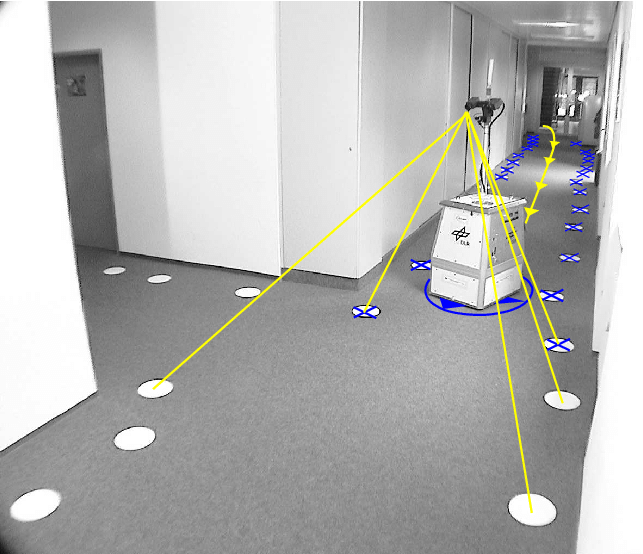
\includegraphics[width=\linewidth]{SLAM_agent} % First image
        \caption[Short caption]{A visual representation of a robot scanning its environment \cite{SLAM_overview}}
        \label{fig:SLAM_agent}
    \end{minipage}\hfill
    \begin{minipage}{0.45\textwidth}
        \centering
        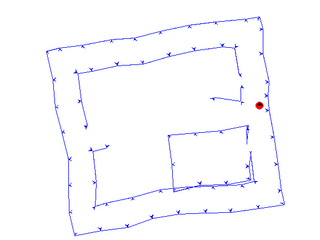
\includegraphics[width=\linewidth]{SLAM_map} % Second image
        \caption[Short caption]{The map (after loop closure) produced by the robot's SLAM algorithm of its environment \cite{SLAM_overview}}
        \label{fig:SLAM_map}
    \end{minipage}
\end{figure}

SLAM (Simultaneous Localisation and Mapping) is a technique used in robotics to create a map of an unknown environment \cite{SLAM_overview}.
It is an important area of research in robotics as it is heavily used in autonomous vehicles, drones and vacuum cleaners;
allowing agents to understand and navigate their environment effectively. Figure \ref{fig:SLAM_agent} shows an example of a
robot scanning its environment, with the sensors visually added to the image.\\
SLAM can be broken down into two sub-problems: localisation and mapping. Localisation is the process of determining the
location of a robot in its environment, whilst mapping is the process of constructing a map of the environment. The maps
are constructed using data collected from sensors, such as cameras and laser scanners; Figure \ref{fig:SLAM_map} shows this.
A lot of existing work in SLAM is based on single robot applications, however, there is a growing interest in multi-agent
SLAM. One of the greatest challenges in SLAM is crossing the simulation to reality gap, as in the real world, sensor
readings are noisy and environments are dynamic, which increases the complexity of the problem.\\
Code implementations of SLAM usually divide the problem into the Front-end and the Back-end \cite{SLAM_components}.
The Front-end is where the agent interprets the environment; it will receive data, which could be in the form of images,
LiDAR scans or other sensor data. The Front-end will then process this data, extracting features and identifying landmarks.
Furthermore, the Front-end will also perform data association, which will compare new features/landmarks to data that has
been previously collected. The Back-end is where the agent will use the data collected from the Front-end to create a map
of the environment and localise itself. There are a number of paradigms which may be used during this process, such as Graph-based
SLAM, Particle filtering and Extended Kalman Filters. By combining the Front-end and the Back-end, the agent will be able to
create an internal representation of its environment and its position in that environment.

\subsection{Background and Evolution of SLAM} % 600 words - currently 513
In the mid 1980s, SLAM concepts were first introduced by Smith and Cheeseman \cite{Early_SLAM}. They initially laid out
the foundations of the problem, which was to be able to reason about the position of an object with potentially inaccurate
information about the environment. Their paper demonstrates a lot of themes which we now associate with SLAM, such as taking
frames (poses) which have an associated positional uncertainty, taking measurements of the environment at each frame and
then using these measurements to identify objects in the environment. Smith and Cheeseman used the Kalman Filter equations
for static-state estimations, and then merged these state estimations to create a representation of the environment.\\
The next major developments in SLAM came shortly after, in the early 90s, from the work of Leonard and Durrant-Whyte \cite{First_EKF}.
In their paper, they identify further challenges in SLAM, such as the data association problem and environment dynamics.
They also outlined one of the traditional problems with SLAM, which is the "chicken and egg" problem. This arises as
to build a useful map, the robot needs to know where it is, and to know where it is, it needs a useful map. To tackle
this, they proposed the use of an Extended Kalman Filter (EKF), which builds on the traditional Kalman Filter equations by
allowing for non-linear state estimations. This was a significant development, as it allowed for the creation of more accurate
maps; however they also concluded that the EKF was not suitable for large-scale environments, as data association becomes
increasingly difficult.\\
Come the 2000s, SLAM had become a well-established area of research, with a number of different paradigms being used to
approach the problem. One of which was FastSLAM, which was developed by Michael Montemerlo and Sebastian Thrun \cite{FastSLAM}.
FastSLAM was an attempt to solve one of the fundamental flaws of EKF SLAM, which was scalability. FastSLAM works by using
a particle filter to estimate the robot's pose, and then constructs a map of the environment using these poses. A particle filter is
a probabalistic technique used to estimate the robots position, which works by having a set of particles randomly distributed
across the environment, which represent possible positions the robot could be in. As the robot moves, the particles are adjusted
based on measurements from the robots sensors; the position of the robot is then estimated by taking the average of the particles.
FastSLAM main strengths are its ability to handle large environments and improve the computational complexity of EFK SLAM, however
it's weaknesses are that it is not as accurate as EKF SLAM and it struggles with dynamic environments.\\

\begin{figure}[h]
    \centering
    \begin{minipage}{0.8\textwidth}
        \centering
        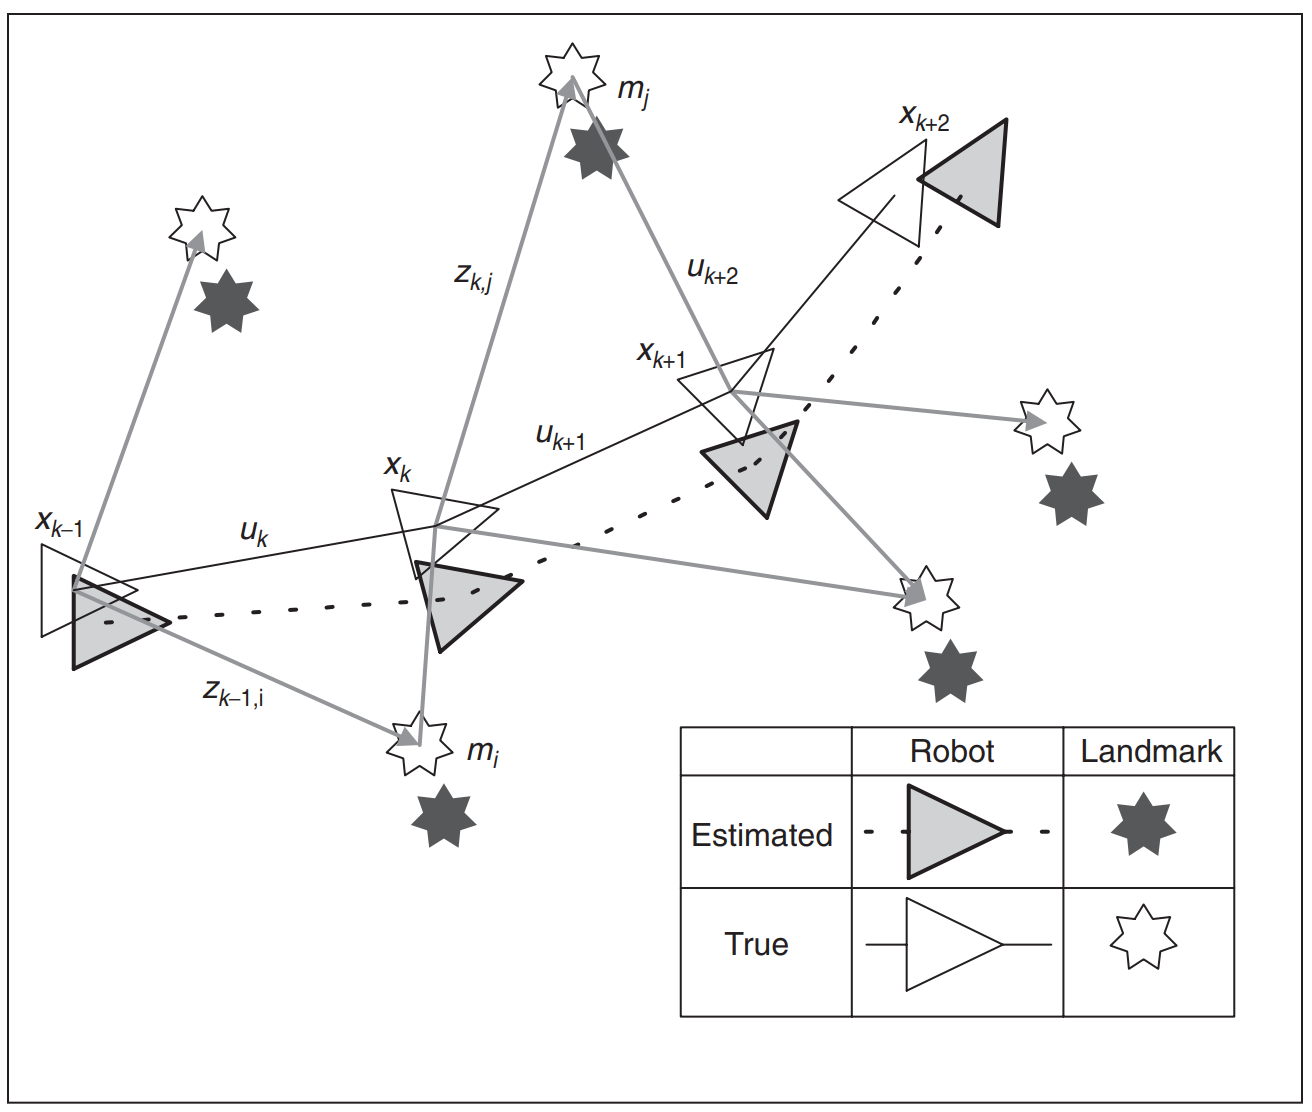
\includegraphics[width=\linewidth]{SLAM_problem} % First image
        \caption[Short caption]{Formal representation of the SLAM problem. \cite{SLAM_summary}}
        \label{fig:SLAM_problem}
    \end{minipage}\hfill
\end{figure}

Finally, in 2006 Durrant-Whyte and Bailey wrote a significant paper outlining the future of SLAM \cite{SLAM_summary}. They started by
discussing existing approaches to the problem and then formally outlining the SLAM problem, shown in Figure \ref{fig:SLAM_problem}. They
then went into further detail on how both EFK SLAM and FastSLAM work, and then discussed the limitations of each approach. They also
wrote a second paper, discussing the future of SLAM, including multi-agent SLAM, 3D SLAM and Dynamic environments \cite{Further_SLAM}.


\subsection{Technical Frameworks and Models} % 800 words - currently 285
\subsubsection{Mapping techniques}
%- grid maps
%- feature-based maps
%- semantic maps
\begin{figure}[h]
    \centering
     \begin{minipage}{0.4\textwidth}
        \centering
        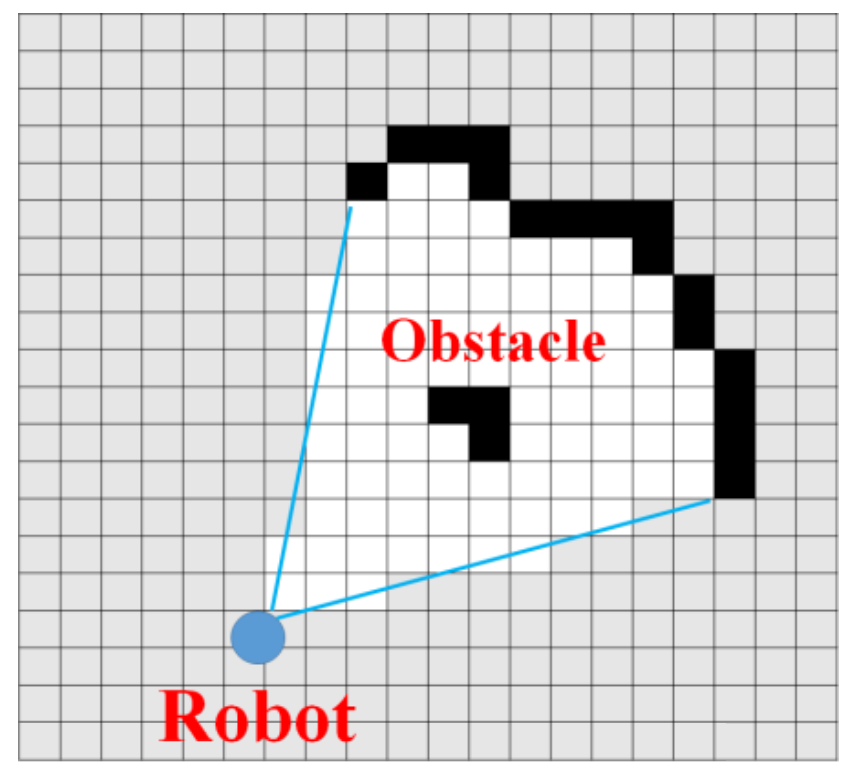
\includegraphics[width=\linewidth]{occupancy_grid} % First image
        \caption[Short caption]{Simple visualization of an occupancy grids \cite{occupancy_grid}}
        \label{fig:simple_occ_grid}
    \end{minipage}\hfill
    \begin{minipage}{0.4\textwidth}
        \centering
        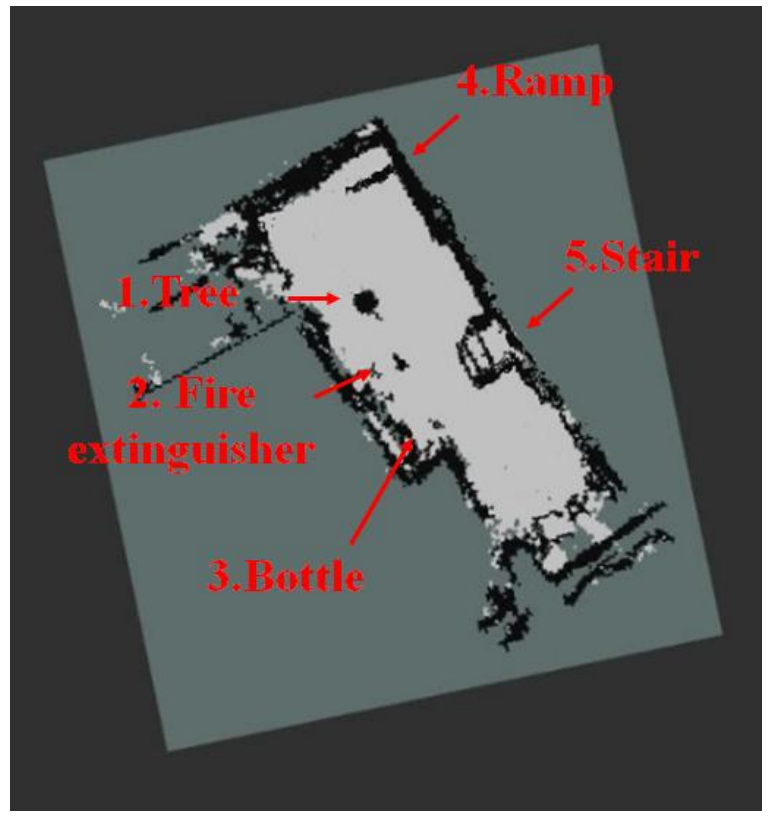
\includegraphics[width=\linewidth]{complex_occ_grid} % Second image
        \caption[Short caption]{Complex example of occupancy grid in practice \cite{occupancy_grid}}
        \label{fig:complex_occ_grid}
    \end{minipage}
\end{figure}

Mapping techniques are used by the agent to create a representation of its environment. There are a number of different mapping techniques
commonly used in SLAM, such as grid maps, feature-based maps and semantic maps. Grid maps, or occupancy maps, are the most common
type of map used in SLAM, as they are easy to implement and computationally efficient. They are typically represented as a 2D array, which
simply stores a binary value for each cell, which represents whether the cell is occupied or not. Figure \ref{fig:simple_occ_grid} shows a simple
example of an occupancy grid, where the black cells represent occupied space and the white cells represent free space. Figure \ref{fig:complex_occ_grid}
demonstrates how an occupancy grid can be used to represent a more complex environment, such as the experiment environment used by Nam
et al \cite{occupancy_grid}. Occupancy grids are typically implemented in conjunction with distance sensors, such as LiDAR - this allows the
agent to measure the distances to multiple points in the environment, which can then be used to update the occupancy grid. \\
Feature-based maps are another common type of map used in SLAM. They work by having the agent detect features in the environment, such as
walls, corners and edges. These features are then used to define landmarks, which are then used to create a map of the environment. Landmarks
are distinct features in the environment which can be used to localise the agent; a common metaphor used to describe landmarks is a distinctive
skyscraper in a city, like the Shard in London, which you could use to figure out your location. Feature-based maps are also implemented with
distance sensors, as the agent can use points detected by the sensor to detect features. \\



Finally, semantic maps are a more recent addition to SLAM, which work by allowing the agent to detect and classify objects in the environment.




\subsubsection{Localization techniques}
- Kalman Filters
- Particle Filters
- visual odometry


\subsubsection{Sensor technologies}
- LiDAR
- Cameras
- Inertial Measurement Units

\subsection{Algorithms and Implementations} % 700 words
\subsubsection{Algorithms}
- EKF SLAM
- FastSLAM
- ORB-SLAM
\subsubsection{Software}
- GMapping
- ROS
\subsubsection{Challenges}
- Feature extraction in dynamic env
- Scalability
- Computational efficiency

\subsection{Real-world Applications and Case Studies} % 600 words
Real world applications:
- Autonomous vehicles
- Drones
- Vacuum cleaners
- Search and rescue
- indoor, outdoor, underwater and airbourne

%deleted shit
%\subsection{Graph-based SLAM}
%Graph-based SLAM is a technique used to create a map of an environment, by using a graph to represent the environment. It
%works by having a robot move around its environment, whilst taking measurements of its surroundings. These measurements
%are usually received by a sensor, such as a camera or laser scanner. The robot then uses these measurements to create a
%plot of where objects may be, by combining the measurements from sensors with its memory of the route it has taken. This
%technique is used in many applications, both in research and in the real world.\\
%One limitation of graph-based SLAM is that it is computationally expensive, as it requires a lot of memory to store the
%sensor readings. Also, it is not very scalable, as the more sensors that are added, the more memory is required. Another
%limitation is that it cannot always be reliable, as the algorithm depends heavily on detecting loop closures, which when
%not detected, can lead to a lot of errors in the map. This, combined with even the slightest inaccuracy from sensors/motors
%makes it difficult to apply to the real world.
%
%\subsection{Particle Filters}
%Another technique used in SLAM is particle filters. Particle filters, also known as Monte Carlo localisation, is a probabalistic
%technique used to estimate the localisation of a robot in its environment. It starts with a set of particles randomly distributed
%across the environment, which represent possible locations of the robot. Each particle has an associated weight, representing the
%probability that the particle is the true location of the robot. As the robot moves around the environment, the particles weights
%are then updated based on an algorithm which takes the robots sensors as input. Overall, this technique is very effective, as it
%is able to localise the robot in its environment, even when the environment is dynamic. Also, this process is highly parallelisable,
%as each particle can be updated independently; which makes this a viable solution for real-world applications. However, particle
%filters are susceptible to the "curse of dimensionality", which means that as the number of dimensions increases, the problem's
%complexity rapidly increases.
%
%\subsection{Swarm}
%Swarm robotics is a discipline which studies the coordination of large numbers of robots. It is largely inspired by biology,
%where social organisms achieve complex behaviours through simple interactions with each other and the environment. Swarm
%robotics is an important area of research in robotics, as it has many applications, such as search and rescue, exploration
%and mapping.\\
%One of the benefits of swarm robotics is the scalability and flexibility of the system. This is because the system is
%decentralized, meaning that each agent is able to make decisions independently. This allows for repeatability, as the system
%can be scaled up or down simply by adding or removing agents. Also, it allows for flexibility, as the system can be adapted
%to different environments, as each agent is able to make decisions based on its surroundings.\\
%One of the biggest challenges in swarm robotics is the simulation to reality gap. This is because in simulation, the agents
%are able to easily share information with each other, whilst in the real world, this is more challenging. Furthermore, swarm
%robotics struggles with more complex environments, like outdoors. As a result, swarm robotics still has a lot of room for
%research and development.
%
%\subsection{Random Walks}
%Random walk exploration in the context of swarm mapping is a technique where agents individually map an environment, using
%methods like Graph-based SLAM, Particle Filters, etc. and them combine their findings to a single global map; this is an
%example of a centralised system.\\
%A example of an implementation of random walk exploration is Brownian motion, which is a physics-inspired
%approach. It works by applying a random force to each agent, which determines its direction. The agents then move in this
%direction until they detect an obstacle, at which point they will change direction. This process is repeated until the
%environment is fully mapped. There is randomness provided from the environment, through detecting other agents or obstacles,
%and randomness in motion, as each path is determined by a random force. Overall, collective behaviour emerges from these simple
%rules, which lead to a global behaviour which efficiently maps an environment.\\
%One of the biggest drawbacks of this approach is that it is not scalable, as the agents are not able to communicate their
%maps to each other, which can lead to a lot of redundant exploration. This is because equally, sharing their maps with each
%other would be very computationally expensive. Also, another limitation is that this approach doesn't guarantee effiency.
%This is because of the inherent randomness, which means areas of the environment may be unexplored.\\

%Requirements Analysis

\section{Requirements Analysis}
Table~\ref{tab:requirements_table} shows the requirements for my project, along with their justification. Initially, I will
create a simulation interface, where the user can see the agents, the environment and a representation of the agents internal
map. After I will work towards implementing single-agent and multi-agent SLAM algorithms. I have also added a couple optional
requirements, which can be carried out should time permit but are not critical towards the success of the project.\\
When creating the simulation interface, I will be using the Python programming language, along with the PyGame library. This
will abstract away a lot of the complexity of creating a graphical user interface, allowing me to focus on the core functionality.
I will also use various other scientific python libraries throughout my project, such as NumPy, SciPy and Matplotlib.\\

\begin{table}[H]
    \centering
    \begin{tabular}{|p{0.03\linewidth}|p{0.2\linewidth}|p{0.6\linewidth}|}
        \hline
        \textbf{ID} &
        \textbf{Requirement} &
        \textbf{Justification}\\
        \hline
        \textbf{1} &
        Simulation Interface &
        A graphical user interface will allow me to visually see the agents behaviours, which will aid de-bugging. It will
        also help understand the algorithms in further detail by allowing me to see how they work live.\\
        \hline
        \textbf{2} &
        Single-agent SLAM &
        Implementing a single-agent SLAM algorithm will help provide the required knowledge to tackle the larger challenge
        of multi-agent SLAM. It will also give me benchmark figures to compare my multi-agent SLAM to when evaluating my project.\\
        \hline
        \textbf{3} &
        Multi-agent SLAM &
        This is the main goal of my project. Implementing multi-agent SLAM algorithm will allow me to explore the challenges of
        navigation and exploration.\\
        \hline
        \textbf{4} &
        Evaluation Metrics Integration &
        This will allow me to analyse the performance of my algorithm and make improvements. This requirement includes adding
        functionality to create graphs and charts, which will be used to visualise performance.\\
        \hline
    \end{tabular}
    \caption{Table of requirements and their justification}\label{tab:requirements_table}
\end{table}\\

Along with this table of requirements, there will also be a number of opportunities for optional extensions, should time permit.
These include:
\begin{itemize}
    \item Implementing physical robots.
    \item User interface enhancements, such as adding being able to view each individual agents internal map.
\end{itemize}

\pagebreak

\section{Project Plan}
\begin{figure}[H]
    \centering
    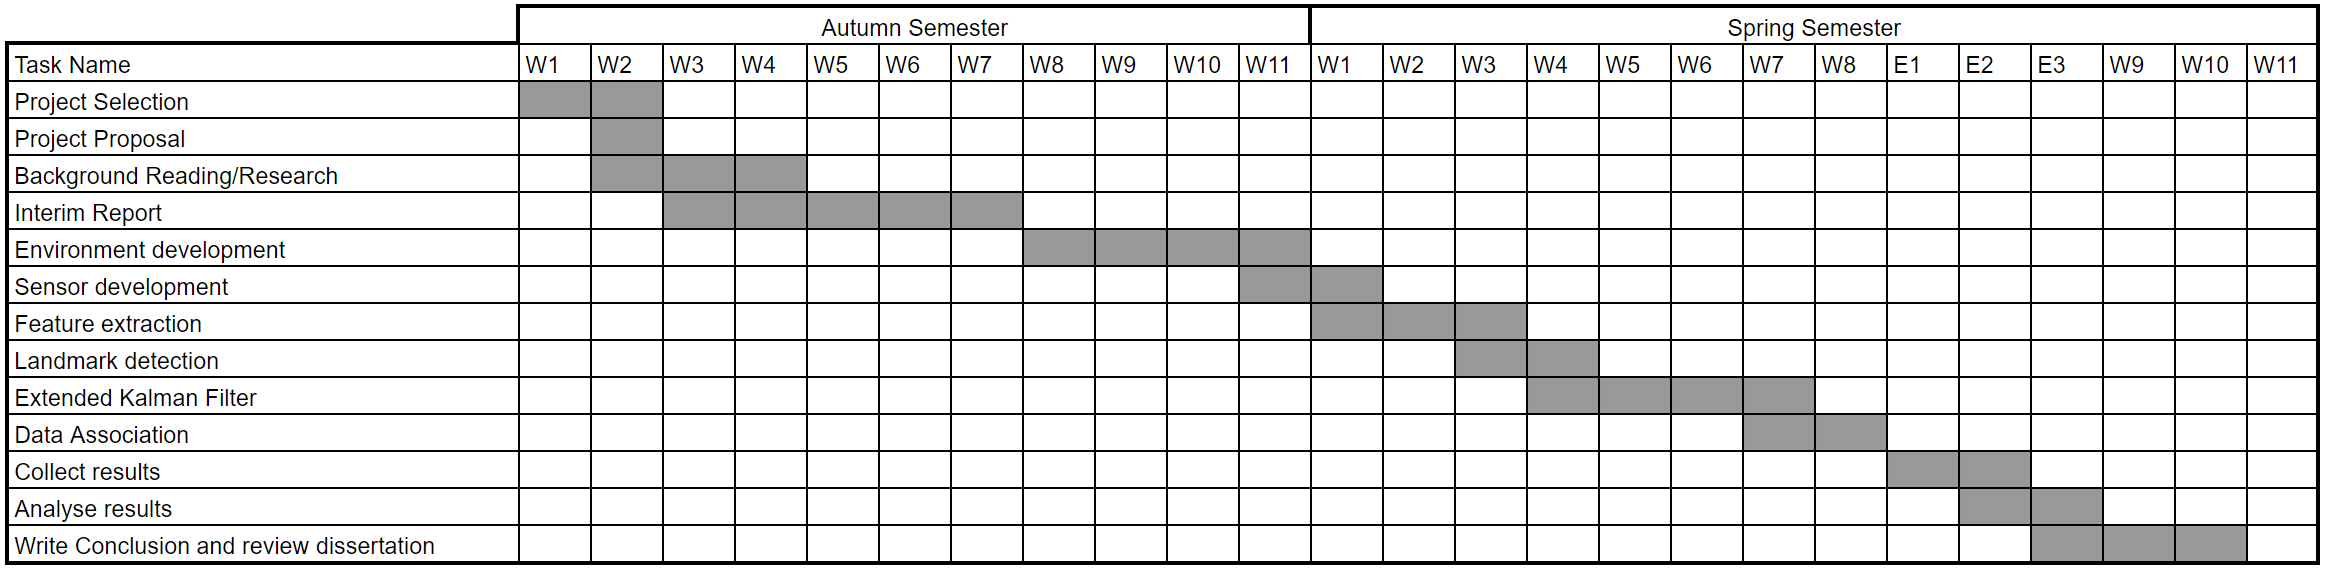
\includegraphics[width=0.8\linewidth]{gantt_chart.png}
    \caption{Gantt chart showing the project plan}
    \label{fig:gantt_chart}
\end{figure}
The execution of my project will be split into various phases, where each phase will focus on an area of development. The
majority of the project will be software development, therefore I have chosen to split this process into various stages. Figure
\ref{fig:gantt_chart} shows the project plan, where the grey bars represent the time spent at each phase. Should my project
overrun, I will have contingency time built into both the Christmas break and prior to the due date, which is currently unaccounted
for in the project plan.\\

\subsection{Phase 1 - Research and Planning}
The first phase of my project involves researching and planning. During this period I will create a project proposal,
research single and multi-agent SLAM algorithms, and write my interim report. This phase will be completed by week 7. It is
important to carry out this phase as it provides structure for the whole project, which will help ensure that the project is
completed on time.

\subsection{Phase 2 - Environment Development}
The second phase of my project will be to develop the simulation environment. This will involve creating a graphical user
interface, using the PyGame library, where the user can see the agent, the environment and a representation of the agents
internal map. This phase will be completed by week 11 - putting me in a good place to work on implementing SLAM algorithms
after the Christmas break.

\subsection{Phase 3 - Single-agent SLAM}
The third phase of my project will be to implement a SLAM algorithm on a single agent system. This will involve implementing
graph-based SLAM, mentioned in my related work section. The algorithm will work by having the agent move around its environment,
whilst taking measurements of its surroundings. These measurements will then be used to predict where objects may be, through
feature extraction. Then, the features detected will be combined to define landmarks, which will be used to create a map of
the environment. Finally, once the algorithm has been implemented, I will create a simple agent which will move around the
environment, using a random walk algorithm. I aim to complete this phase by the end of week 4 of the Spring semester.

\subsection{Phase 4 - Multi-agent SLAM}
In the fourth phase of my project, I will implement a multi-agent SLAM. This will involve creating a centralized multi-agent
SLAM algorithm, where the agents individually collect data and then feed to a global map. To achieve this, I will need to
modify my single-agent SLAM algorithm to firstly allow for a central server to exist, and then I will need to implement a
communication protocol between the agents and the server. To create a complete map, the server will need to combine the maps
from each agent; implementing cross-agent feature matching. The server will also need to have a mechanism which resolves conflicts
in data association, for example, when two agents have conflicting information about a landmark's position. This phase needs
to be completed by week 8 of the Spring semester, which allows for a reasonable amount of time to work on the final report.


\subsection{Phase 5 - Analysis and Conclusion}
I will start the final phase of my project during the Easter break, where I will collect data which will be used to analyse
the performance of the algorithm. I will then use this data to create a series of graphs and charts, which will be used to
visualise performance and draw conclusions. After, a lot of time will be spent writing up my findings and analysing the performance
of the algorithms. Finally, I will conclude my project by writing a conclusion, which will summarise my findings and discuss
potential future work. Prior to submitting my report, I will also spend time proofreading and editing my work.


\section{Professional and Ethical Considerations}
My project maintains compliance towards all ethical considerations, as there is minimal external involvement from
humans. The majority of my project will be carried out in simulation, therefore no ethical approval is required. Should
my project progress to physically implementing agents, considerations such as safety around the robots, will be considered.
All tests will be carried out in an environment where people cannot be hit, therefore mitigating any trip hazards.\\

To ensure all elements of the BCS code of conduct are met, I have summarised each section and how I meet certain criteria. \\
\subsection{Public Interest}
As mentioned previously, my project has due regard for public health, as there is minimal external involvement from humans.
Furthermore, no major privacy, security or wellbeing considerations are required due to the nature of this project. Third parties
will be respected throughout the project with consistent citations and there will be no discrimination against anybody involved.
Finally, I will promote equal access to the benefits of IT by open-sourcing my research once I have graduated. This will be accessible
on my Github profile: \href{https://github.com/CharlieAnthony/}{https://github.com/CharlieAnthony/} \\
\subsection{Professional Competence and Integrity}
My project is within my professional competence, as it significantly relies upon knowledge obtained from modules such as "Acquired
Intelligence and Adaptive Behaviour" and "Fundamentals of Machine Learning." Furthermore, I will develop my professional knowledge,
skills and competence through communicating with my supervisor and ensuring all relevant gaps in knowledge are explored through
reading extensively. As part of my background reading, I have made myself familiar with the BCS code of conduct and surrounding
legistlation. I will comply with this throughout when carrying out my professional responsibilities. There will also
be no unethical inducements offered or accepted throughout the project. \\
\subsection{Duty to Relevant Authority}
As the relevant authority will be the University of Sussex, I will comply with all relevant codes of conduct and legislation. I
will exercise my professional judgement at all times, including avoidance of any situation that may give rise to a conflict of
interest between myself and the university. I will also make it my responsibility to ensure all colleagues work is properly
referenced in a bibliography at the end of my dissertation. \\
\subsection{Duty to the Profession}
Finally, I accept my duty to uphold the reputation of the profession. I will work to the best of my ability to ensure my project
is complete to the highest possible standard. As mentioned previously, I will seek to improve professional standards through
communication with my supervisor. This dissertation will be written with integrity and respect towards all members of BCS and colleagues
of the profession. \\


%Related Work

\section{Methods}

\subsection{Single-Agent SLAM}

\subsubsection{Feature Extraction}
Feature extraction is the process of detecting and extracting features from sensor data. In the context of SLAM, features
are points of interest in the environment, such as corners, edges and lines. These features can then be used to create a map
of the environment. There are many different techniques for feature extraction, such as the Harris corner detector and the
split-and-merge algorithm. My implementation uses Seeded region growing, which was proposed by Gao et al.
\cite{seeded_region_growing}.\\
Seed segment detection works by observing a set of points from a single sweep. The algorithm starts by fitting a line through
the given points. Then, in order for a seed segment to be further considered, it must satisfy the following two conditions:
\begin{itemize}
    \item The distance between the point and the line must be less than a given threshold.
    \item The distance between the point and it's predicted position must be less than a given threshold.
\end{itemize}
Seed segment detection uses orthogonal line fitting to propose a feature through a set of points, as it is more effective
than using traditional methods, such as standard least square fitting; this is due to the nature of least square fitting
which only takes into account the vertical distances of each point.\\
After, the algorithm applies region growing, which helps create line segments; which will then become our features. The
region growing works by examining neighbouring points and adding them to the line segment if they satisfy the same conditions.
This process is repeated until no more points can be added to the line segment.\\

\subsubsection{Identifying Landmarks}
\subsubsection{Data Association}
\subsubsection{Pose Graph}
\subsubsection{Graph Optimisation}


\section{Appendices}

\subsection{Supervisor Meetings}    % 720 words

\subsubsection{Meeting 1 - 11/10/2023}
Discussed on the project idea and potential directions to take. Discussed the possibility of implementing physical agents,
challenges that may occur and potential ways of implementing swarm algorithms. Need to focus on researching SLAM and swarm
and looking into existing resources.
\subsubsection{Meeting 2 - 27/10/2023}
Discussed potential algorithms, such as particle filters and graph-based SLAM. We also discussed the logistics of the project,
ensuring that it remains both realistic and achievable. We also discussed the possibility of implementing physical agents,
and where relevant resources could be found.
\subsubsection{Meeting 3 - 14/11/2023}
Started with feedback on the interim report - discussing the structure and content. After we discussed how the project will
move forward and the next steps to take. Given the interim report is now complete, we can focus mainly on development, following
the project plan. As I have already developed a basic simulation interface, I can now move onto implementing my first SLAM algorithm.
\subsubsection{Meeting 4 - 08/12/2023}
In this meeting, we turned to ironing out the specifics of the implementation - including looking at existing resources, like
Enki, and concepts that need to be considered, such as Differential Turning. The goal of this meeting was to guide me into
starting to create my environment and first SLAM algorithm, which will be implemented over the christmas break.
\subsubsection{Meeting 5 - 02/02/2024}
We firstly caught up on progress made over the christmas break. After, we started to look forward to the next steps of the project,
discussing the projects overall direction and the next steps to take. One notable suggestion was the move away from swarm algorithms
and perhaps the move towards multi-agent SLAM, as this would be more achievable in the time frame. Finally, we discussed how I
should manage my time towards the end of the project and how I could start working on my dissertation.
\subsubsection{Meeting 6 - 09/02/2024}
Started with me demonstrating my current progress, with my environment working, LIDAR sensor appropriately implemented and
my work-in-progress feature detection. We discussed then how I could approach landmark detection and how I planned on implementing
it. We ended the meeting with clearing up questions regarding the project presentation, poster competition and submission.
\subsubsection{Meeting 7 - 16/02/2024}
We discussed how my project was going; talking about feature extraction and landmark detection. As I had been having troubles
with bugs in the previous week, Chris suggested spending more time writing test cases. We then discussed how I should approach
writing the final report; considering structure and content. We agreed that there are parts of the report that I could start
now, such as my literature review and methodology used in feature detection and landmark detection.
\subsubsection{Meeting 8 - 23/02/2024}
Started with showing my progress on landmark detection and randon walk exploration. We then discussed different exploration
algorithms that could be used, as random walk exploration isn't efficient. We discussed creating some form of wall-avoidance
navigation, which would be far more efficient. We then reviewed my plan and reflected on how progress was going. We both
agreed that progress isn't as fast as we would like, but we are still on track to complete the project on time.
\subsubsection{Meeting 9 - 29/02/2024}
We had a quick online meeting this week; discussing where the project is and the next steps. We started by talking about
my implementations of exploration strategies and how I could improve them. We then discussed evaluation metrics and how I
could gather and present data. Finally, we talked about how I could approach multi-agent SLAM, as it's an area I am concerned
about due to it's complexity.
\subsubsection{Meeting 10 - 15/03/2024}
This meeting was a clear turning point in the project. As progress hadn't proceeded as expected, we discussed the scope of
the project and how it could be adjusted to ensure that I could complete it on time. We agreed that I should focus on the single-agent
components of SLAM, as they are the most important parts of my project. We also discussed how I could approach the final report -
including changes that would need to be made to adhere to the new project scope. Finally, we discussed in further detail how I could
gather data for my analysis and how I could present it.

\subsection{Project Proposal}
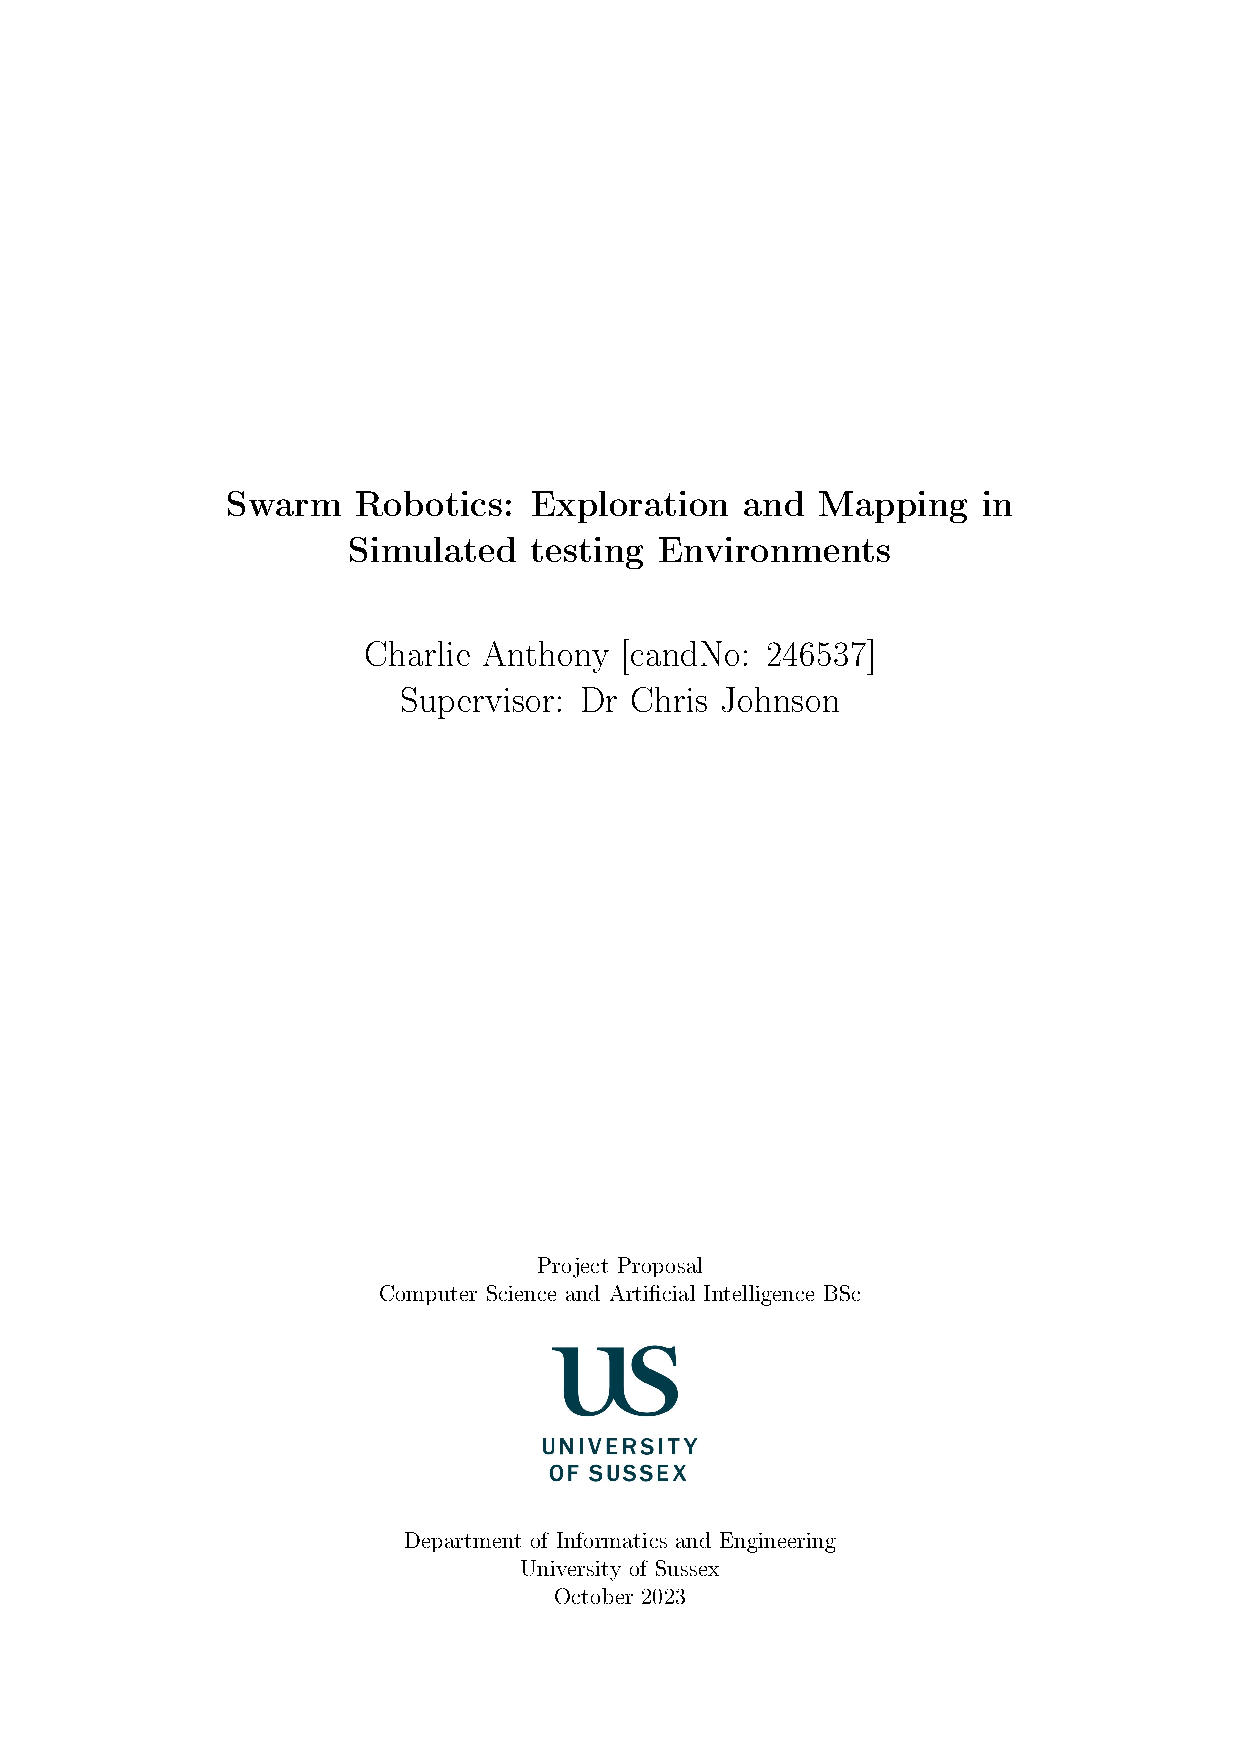
\includepdf[pages=-]{ProjectProposal.pdf}

%References
\section{References}

\begin{thebibliography}{9}

    \bibitem{SLAM_overview}
    Frese, U., Wagner, R. and Röfer, T. (2010). A SLAM Overview from a User’s Perspective.
    \textit{KI - Künstliche Intelligenz}, 24(3), pp.191–198.
    \href{http://dx.doi.org/10.1007/s13218-010-0040-4}{http://dx.doi.org/10.1007/s13218-010-0040-4}

    \bibitem{SLAM_components}
    Alsadik, B. and Karam, S. (2021) The Simultaneous Localization and Mapping (SLAM)-An Overview.
    \textit{Journal of Applied Science and Technology Trends, 2(02), pp. 147 - 158.}
    \href{https://doi.org/10.38094/jastt204117}{https://doi.org/10.38094/jastt204117}

    \bibitem{Early_SLAM}
    Smith, R.C.; Cheeseman, P. (1986). "On the Representation and Estimation of Spatial Uncertainty".
    \textit{The International Journal of Robotics Research. 5 (4): 56–68.}
    \href{https://doi.org/10.1177/027836498600500404}{https://doi.org/10.1177/027836498600500404}

    \bibitem{First_EKF}
    J. J. Leonard and H. F. Durrant-Whyte, "Simultaneous map building and localization for an autonomous mobile robot,"
    \textit{Proceedings IROS '91:IEEE/RSJ International Workshop on Intelligent Robots and Systems '91, Osaka, Japan, 1991, pp. 1442-1447 vol.3,}
    \href{https://doi.org/10.1109/IROS.1991.174711}{https://doi.org/10.1109/IROS.1991.174711}

    \bibitem{FastSLAM}
    Montemerlo, M., Thrun, S., Koller, D. and Wegbreit, B., 2002. "FastSLAM: A factored solution to the simultaneous localization and mapping problem,"
    \textit{Proceedings of the AAAI National Conference on Artificial Intelligence. pp. 593-598}.

    \bibitem{SLAM_summary}
    Durrant-Whyte, H. and Bailey, T. (2006). "Simultaneous localization and mapping: part I",
    \textit{IEEE Robotics & Automation Magazine, [online] 13(2), pp.99–110}.
    \href{https://doi.org/10.1109/mra.2006.1638022}{https://doi.org/10.1109/mra.2006.1638022}

    \bibitem{Further_SLAM}
    T. Bailey and H. Durrant-Whyte, "Simultaneous localization and mapping (SLAM): part II,"
    \textit{IEEE Robotics & Automation Magazine, vol. 13, no. 3, pp. 108-117, Sept. 2006}.
    \href{https://doi.org/10.1109/MRA.2006.1678144}{https://doi.org/10.1109/MRA.2006.1678144}

    \bibitem{occupancy_grid}
    Nam, Tae & Shim, Jae & Cho, Young. (2017). "A 2.5D Map-Based Mobile Robot Localization via Cooperation of Aerial and Ground Robots",
    \textit{Sensors 17(12): 2730}.
    \href{http://dx.doi.org/10.3390/s17122730}{http://dx.doi.org/10.3390/s17122730}

    \bibitem{C-SLAM}
    Lajoie, P.Y. and Beltrame, G. (2023). Swarm-slam: Sparse decentralized collaborative simultaneous localization and mapping framework for multi-robot systems.
    \textit{arXiv preprint},  arXiv:2301.06230.
    \href{https://doi.org/10.48550/arXiv.2301.06230}{https://doi.org/10.48550/arXiv.2301.06230}

    \bibitem{seeded_region_growing}
    Gao, H., Zhang, X., Fang, Y. and Yuan, J. (2018). A line segment extraction algorithm using laser data based on seeded region growing.
    \textit{ International Journal of Advanced Robotic Systems}, p.172988141875524.
    \href{https://doi.org/10.1177/1729881418755245}{https://doi.org/10.1177/1729881418755245}

\end{thebibliography}



\end{document}


